% $> xelatex spsi.tor.presentacion.tex
% o bien
% $> lualatex spsi.tor.presentacion.tex
\documentclass[spanish]{beamer}

\usepackage{babel}

\usepackage{graphics,tikz}
\usetikzlibrary{automata, positioning, arrows}

\usepackage{pgfplotstable}
\pgfplotsset{compat=1.16}

\usepackage{adjustbox}

\usepackage{enumitem}

%%% FUENTES

\usepackage[no-math]{fontspec}
\setmainfont{Libertinus Serif}
\setsansfont{Libertinus Sans}
\setmonofont{Libertinus Mono}

\usepackage[math-style=TeX]{unicode-math}
\setmathfont{Libertinus Math}

\usepackage{pifont}
\newcommand{\cmark}{\ding{51}}%
\newcommand{\xmark}{\ding{55}}%

%%% COLORES

\definecolor{background}{HTML}{F5F5F4}
\definecolor{foreground}{HTML}{3F3F3F}
\definecolor{strings}{HTML}{ED982C}
\definecolor{operators}{HTML}{CF4818}
\definecolor{identifiers}{HTML}{9A71BA}
\definecolor{keywords}{HTML}{5486C8}
\definecolor{numbers}{HTML}{80951D}
\definecolor{comments}{HTML}{AFAFAF}

%%% LISTINGS

\usepackage{listings}

\lstset{
  numbers=left,
  belowcaptionskip=1\baselineskip,
  basicstyle=\scriptsize\ttfamily\color{foreground},
  keywordstyle=\color{keywords},
  commentstyle=\color{comments},
  stringstyle=\color{strings},
  identifierstyle=\color{identifiers},
  numberstyle=\color{foreground},
  xleftmargin=2em,
  framexleftmargin=1.5em,
  breaklines=true,
  showstringspaces=false,
  tabsize=2
}

% Bibliografía

\usepackage[sorting=none, style=apa, isbn=true]{biblatex}
\DefineBibliographyStrings{spanish}{
  urlseen = {Consultado},
  retrieved = {Consultado},
}
\addbibresource{bibliografia.bib}

%%% AJUSTES DE BEAMER

%\usefonttheme{professionalfonts}

\setbeamertemplate{navigation symbols}{}

\setbeamerfont{title}{series=\bfseries}

%\setbeamertemplate{frametitle}{\color{foreground}\vspace*{1cm}\bfseries\insertframetitle\par\vskip-6pt}
\setbeamerfont{frametitle}{series=\bfseries}
\setbeamercolor{frametitle}{fg=foreground}
\setbeamerfont{framesubtitle}{size=\normalfont\small}
\setbeamercolor{framesubtitle}{fg=foreground}

\setbeamercolor{background canvas}{bg=background}

\setbeamercolor{normal text}{fg=foreground}
\setbeamercolor{alerted text}{fg=foreground}
\setbeamercolor{block title}{fg=foreground}
\setbeamercolor{alerted text}{fg=foreground}

\setbeamercolor{itemize item}{fg=foreground}
\setbeamercolor{enumerate item}{fg=foreground}

\setbeamertemplate{itemize items}[circle]
\setitemize{
  label=\usebeamerfont*{itemize item}
  \usebeamercolor[fg]{itemize item}
  \usebeamertemplate{itemize item}
}

\setbeamercolor*{title}{fg=foreground}
\setbeamercolor{qed symbol}{fg=foreground}

\usebeamercolor[fg]{normal text}

\setbeamertemplate{footline}[frame number]
\setbeamerfont{page number in head/foot}{size=\small}

%%% INFORMACIÓN DEL DOCUMENTO

\title{Curvas elípticas en la criptografía}
\subtitle{Historia de las Matemáticas}
\author{
  Sofía Almeida Bruno \texorpdfstring{\\}{} 
  Antonio Coín Castro \texorpdfstring{\\}{} 
  José María Martín Luque
}
\institute{\normalsize Universidad de Granada}
\date{17 de diciembre de 2019\texorpdfstring{\\}{} \small Curso 2019-2020}

\begin{document}

\maketitle

\begin{frame}{Índice}
  \tableofcontents
\end{frame}

\section{Criptografía}
\begin{frame}{Criptografía}
  \begin{itemize}
    \item Objetivo: transmitir información confidencial a través de un canal inseguro.
    \item Ya en la antigüedad se usaba en contextos bélicos o políticos. Un ejemplo es el \textit{cifrado del César}:
    \[x \mapsto x + 3 \mod 26.\]
    \item En la \textit{era de la información} experimenta una evolución sin precedentes.
    \item Los sistemas actuales basan su seguridad en problemas matemáticos \textit{difíciles} de resolver. 
  \end{itemize}
\end{frame}

\section{Curvas elípticas}
\begin{frame}{Curvas elípticas}{Definición (I)}
  \begin{itemize}
    \item Una \textit{curva elíptica} sobre un cuerpo $K$ es una curva proyectiva no singular $E \subset \mathbb{P}^2(K)$ definida por una ecuación de la forma
    \[ y^2 + a_1xy + a_3y = x^3 +a_2x^2 + a_4x + a_6,\]
    con cada \(a_i \in K\).
    \item Si la característica de \(K\) es distinta de \(2\) y \(3\) podemos simplificar la ecuación, obteniendo la \textit{ecuación de Weierstrass}
    \[y^2 = x^3 + Ax + B,\]
    con \(A, B \in K\).
  \end{itemize}
  
\end{frame}

\begin{frame}{Curvas elípticas}{Definición (II)}
  Se puede comprobar que la curva corta a la recta del infinito en un único punto.
  \[ E = E(K) = \left\{ (x, y) \in K \times K : y^2 = x^3 + Ax + B\right\} \cup \big\{\mathcal{O}\big\}.\]
  \begin{itemize}
    \item \(\mathcal O\) es el punto del infinito con coordenadas homogéneas \([0:1:0]\).
    \item La condición de no singularidad se traduce en \(4A^3 + 27B^2 \neq 0\).
  \end{itemize}
  
\end{frame}

\begin{frame}[fragile]{Curvas elípticas}{Ejemplos}
  \begin{figure}[h]
    \centering
    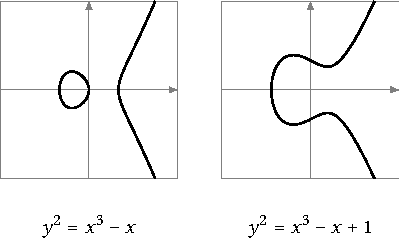
\includegraphics[width=.75\textwidth]{img/ejemplos-curvas}
    \caption{Ejemplos de curvas elípticas sobre $\mathbb{R}$. Basado en \parencite{eichlseder_elliptic_2016}.}
    \label{fig:curva}
  \end{figure}
\end{frame}

\begin{frame}{Suma de puntos (I)}
  % Hablar de:
  % - método algebraico (lo que vamos a contar se hace con ecuaciones)
  % - el método geométrico lo vemos sobre R
  % - las rectas verticales cortan a la curva al menos en el punto del infinito
  \begin{itemize}
    \item Podemos definir una operación suma sobre los puntos de la curva para obtener un grupo abeliano.
    \item El elemento neutro será el punto \(\mathcal{O}\).
    %\item Vamos a ver el método geométrico sobre \(\mathbb R\).
  \end{itemize}
\end{frame}

\begin{frame}{Suma de puntos}
  \begin{figure}[h]
    \centering
    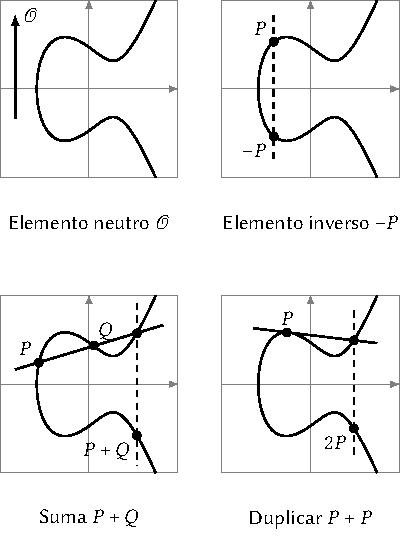
\includegraphics[width=0.65\textwidth]{img/operaciones-curvas}
    \caption{Suma de puntos en curvas elípticas. Basado en  \parencite{eichlseder_elliptic_2016}.}
    \label{fig:operaciones-curvas}
  \end{figure}  
\end{frame}

% TODO: Insertar figuras operaciones

\begin{frame}
  \printbibliography
\end{frame}

\end{document}

